\documentclass[10pt, UKenglish]{beamer}
\usepackage{babel}
\usepackage[utf8]{inputenc}  
\usepackage{geometry}
\usepackage[customcolors]{hf-tikz}
\usepackage[T1]{fontenc}   
\usepackage{tcolorbox}
\usepackage{siunitx}
\usepackage{hyperref}
\usepackage{bookmark}
\usepackage{marvosym}
\usepackage{tikz}
\usepackage{tikz-qtree}
\usepackage{cancel}
\usepackage{todonotes}
\useoutertheme[subsection=false]{smoothbars}
\DeclareSIUnit[number-unit-product = {}]{\inchQ}{\textquotedbl}
\usepackage{amsmath}
\usepackage{amssymb}
\newcommand\hmmax{0} % default 3
% \newcommand\bmmax{0} % default 4
\usepackage{bm} 
\DeclareSIUnit[number-unit-product = {\thinspace}]{\inch}{in}
\usetheme[menuwidth={0.3\paperwidth}]{erlangen}
\usepackage{multicol}
\usepackage{charter}
\setbeamercovered{transparent=20}
\setbeamertemplate{navigation symbols}{}
\sisetup{separate-uncertainty = true}
\usepackage[version=4]{mhchem}
\usepackage{tikz}
\usepackage{hepnames}
\usepackage{soul}
\usepackage{color}
\usepackage{thesis_defs}
\usepackage{subcaption}
\usepackage{xcolor}
\usepackage{enumitem}
\setlist[enumerate]{labelindent=10pt,style=multiline,leftmargin=2.5cm}
\setlist[itemize]{font=$\bullet$\scshape\bfseries}

\usepackage[backend=biber]{biblatex}
\bibliography{bibliography.bib}

\graphicspath{%
  {../../feynman_diagrams/}%
  {./figures_theory/}%
  {./figures_simple/}%
  {./figures_misc/}%
  {./app1/}%
  {./app2/}%
  {./app3/}%
}


\definecolor{color1}{RGB}{33,217,217}
\definecolor{color2}{RGB}{7,61,111}

\newcommand{\lr}{\mathcal{lr}}


\newcounter{totavalue}
\newcounter{parvalue}

\def\aux{1}
\def\radius{9pt}
\def\step{4pt}
\usepackage[absolute,overlay]{textpos}


\newcommand\circcounter{%
\ifnum\inserttotalframenumber<2\relax
\else
  \setcounter{totavalue}{\inserttotalframenumber}
  \setcounter{parvalue}{\insertframenumber}
  \ifnum\inserttotalframenumber>45\relax
    \renewcommand\step{0pt}
  \fi%
  \pgfmathsetmacro{\aux}{360/25}
  \begin{tikzpicture}[remember picture,overlay, rotate=90+\aux]
  \foreach \i in {0,1,...,25}
    \fill[logo_blue] 
      (0,0) -- (-\i*\aux:\radius) arc  (-\i*\aux:-(\i+1)*\aux+\step:\radius) -- cycle;
  \foreach \i in {1,...,\insertframenumber}
    \fill[logo_grey] 
      (0,0) -- (-\i*\aux:\radius) arc  (-\i*\aux:-(\i+1)*\aux+\step:\radius) -- cycle;
  \fill[white] circle (\radius/1.3);
  \node at (0,0) {\small\insertframenumber}; 
  \end{tikzpicture}%
\fi%
}


\usepackage{eso-pic,picture}



\begin{document} 

\title[Bachelorvortrag]{Categorical neural networks for background separation in the analysis of single top-quark production in association with a Higgs boson}
\subtitle{15th of September 2021}
\author{Christian Kirfel}
%\institute{Universtität Bonn}
        



\begin{frame}[plain]
\vspace{0.0cm}
  \titlepage
      \AddToShipoutPictureFG*{%
    \AtPageUpperLeft{%
      \put(8.7cm,-9.6cm){

\includegraphics[scale=0.03]{original_logo.jpg}
\makebox(0,0)[lt]{}%
      }%
    }%
  }%
    \AddToShipoutPictureFG*{%
    \AtPageUpperLeft{%
      \put(0.0cm,-9.6cm){
%\includegraphics[scale=0.17]{atlas_gay.png}

\includegraphics[scale=0.17]{ATLAS-Logo-Ref-RGB-H_0.jpg}
\makebox(0,0)[lt]{}%
      }%
    }%
  }%
\end{frame}
\addtobeamertemplate{navigation symbols}{\vspace*{0.8cm}\hfill\circcounter\hspace*{0.7cm}}

\section{Neural Networks}
\section{Binary}
\begin{frame}
    \begin{center}
        \Huge \tHq \\ A binary classifier
    \end{center}
\end{frame}

\begin{frame}{Hyperparameters}
  \begin{itemize}
    \item Optimised by small grid search
  \end{itemize}
    \begin{table}[]
    \begin{tabular}{|l|l|}
    \hline
    Hyperparameter          &     Setting              \\ \hline
    Model                   &     Binary          \\ \hline
    Nodes                   &     120                  \\ \hline
    Layers                  &     6                    \\ \hline
    Dropout                 &     0.65                 \\ \hline
    Batchnormalisation      &     On                   \\ \hline
    Activation              &     elu                  \\ \hline
    Output activation       &     sigmoid              \\ \hline
    Batch size              &     1000                 \\ \hline
    Optimisation            &     Adam                 \\ \hline
    Weight Initialisation   &     Lecun Normalisation  \\ \hline
    K-folds                 &     4                    \\ \hline
    \end{tabular}
    \end{table}
\end{frame}

\begin{frame}{Results}
    \begin{columns}
        \begin{column}{0.5\textwidth}
          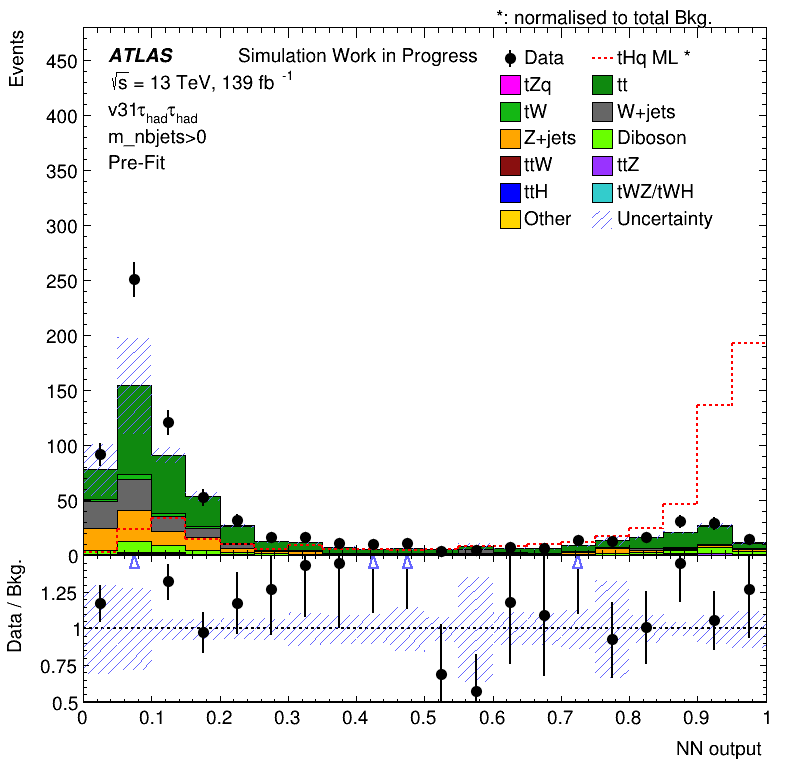
\includegraphics[width=0.82\textwidth]{response_binary}
          \begin{itemize}
            \item Decent separation
            \item Stable agreement
          \end{itemize}
        \end{column}
        \begin{column}{0.5\textwidth}
          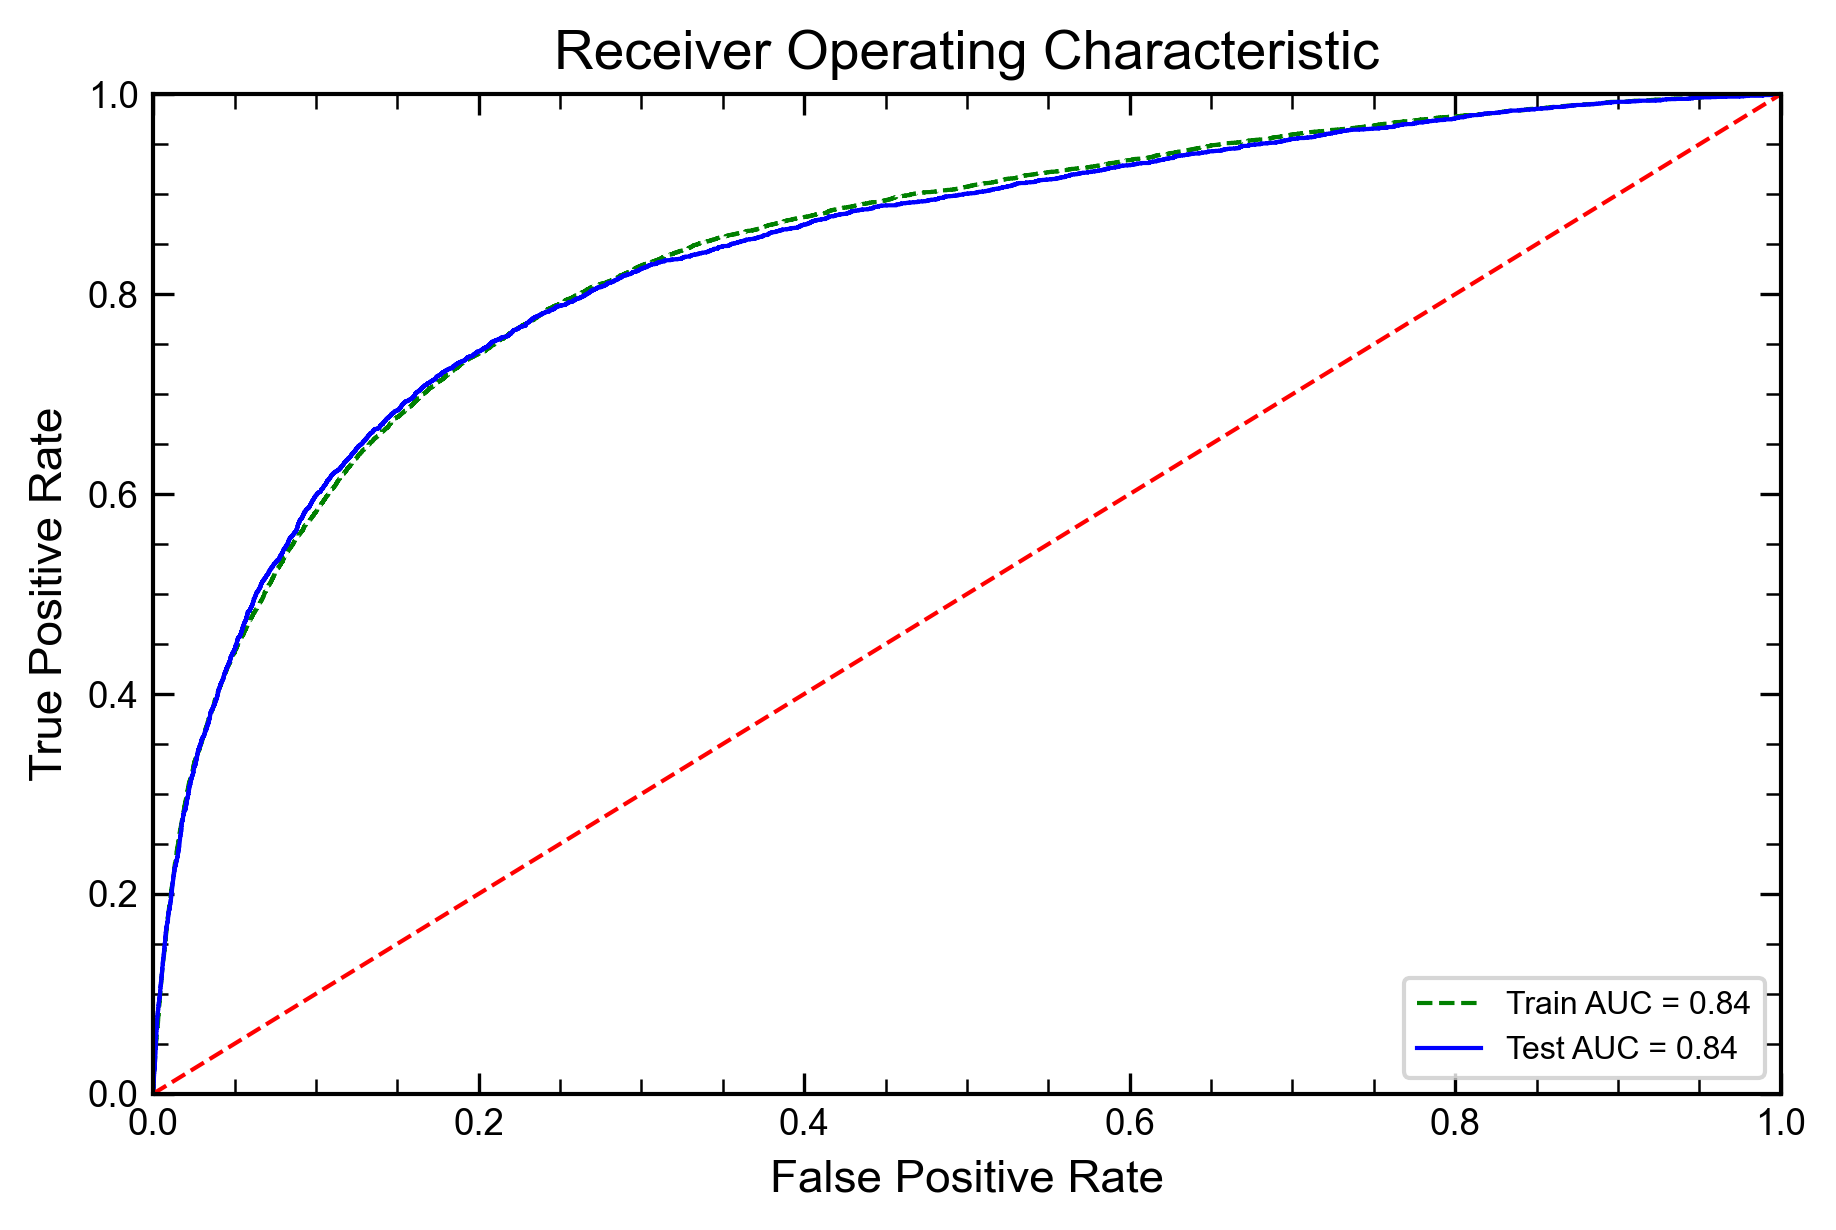
\includegraphics[width=0.84\textwidth]{ROC_binary}
          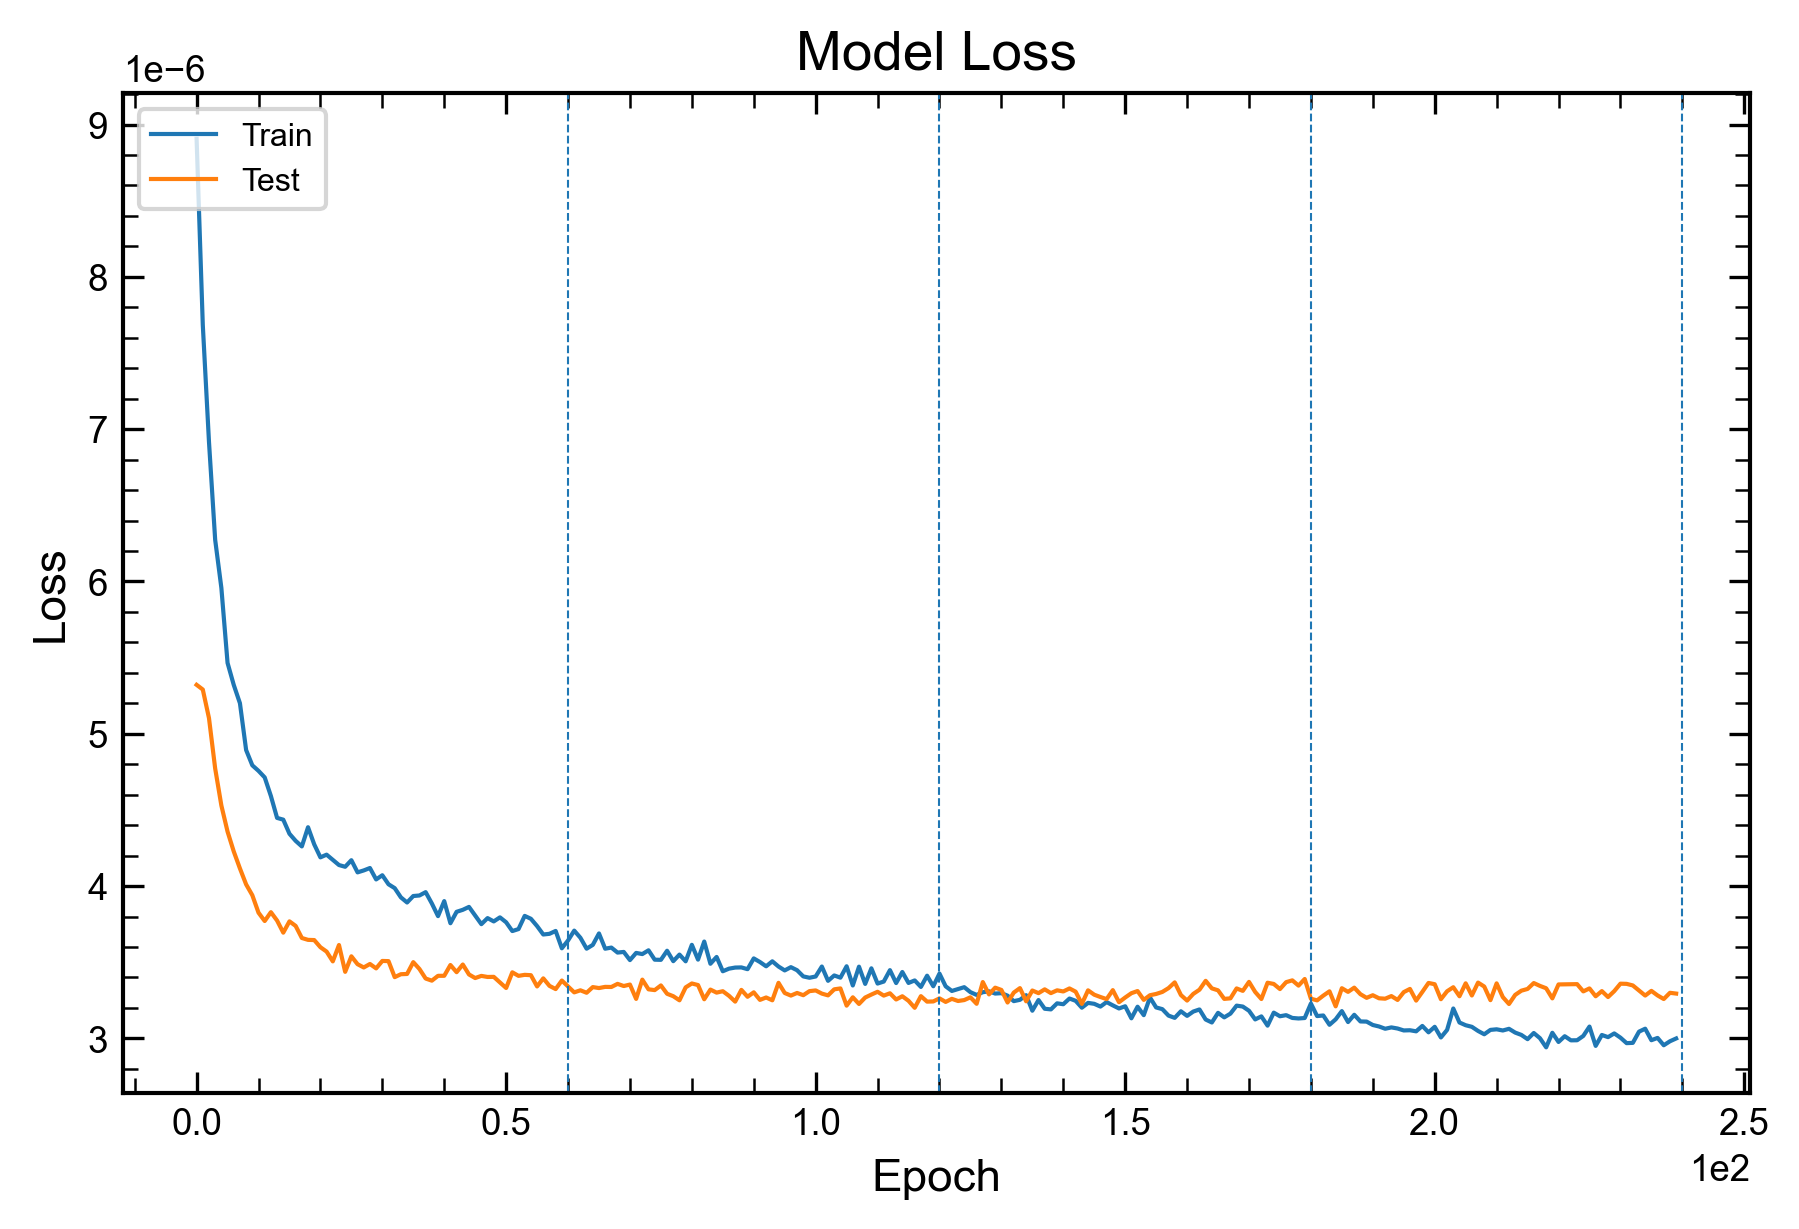
\includegraphics[width=0.84\textwidth]{loss_binary}
        \end{column}
    \end{columns}    
\end{frame}

\begin{frame}
    \begin{center}
        \Huge \tHq \\ A closer look
    \end{center}
\end{frame}

\begin{frame}{The ROC curve}
  \centering 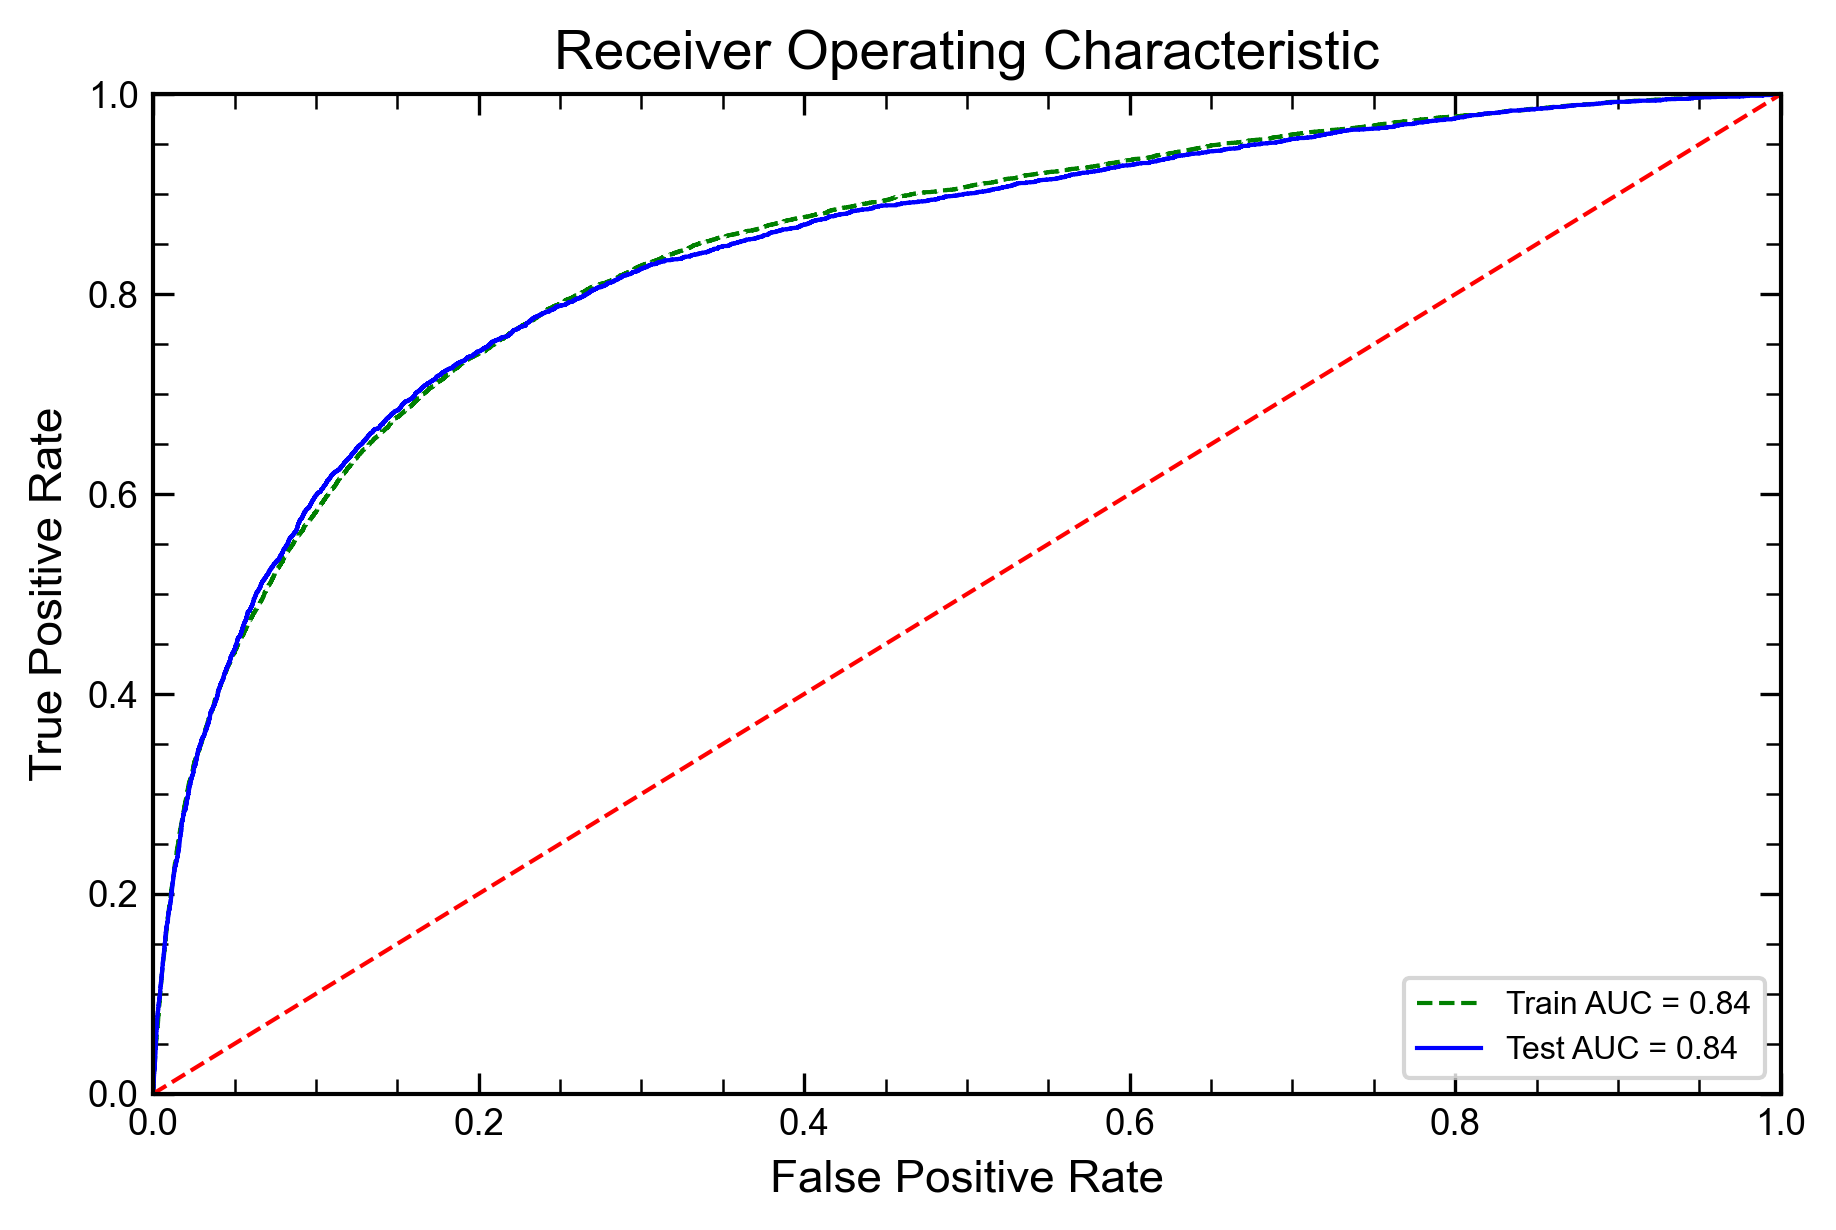
\includegraphics[width=0.8\textwidth]{ROC_binary}
  \begin{itemize}
    \item AUC = Are Under the Curve
    \item Good estimator for model quality
  \end{itemize}
\end{frame}

\begin{frame}{The loss curve}
  \centering 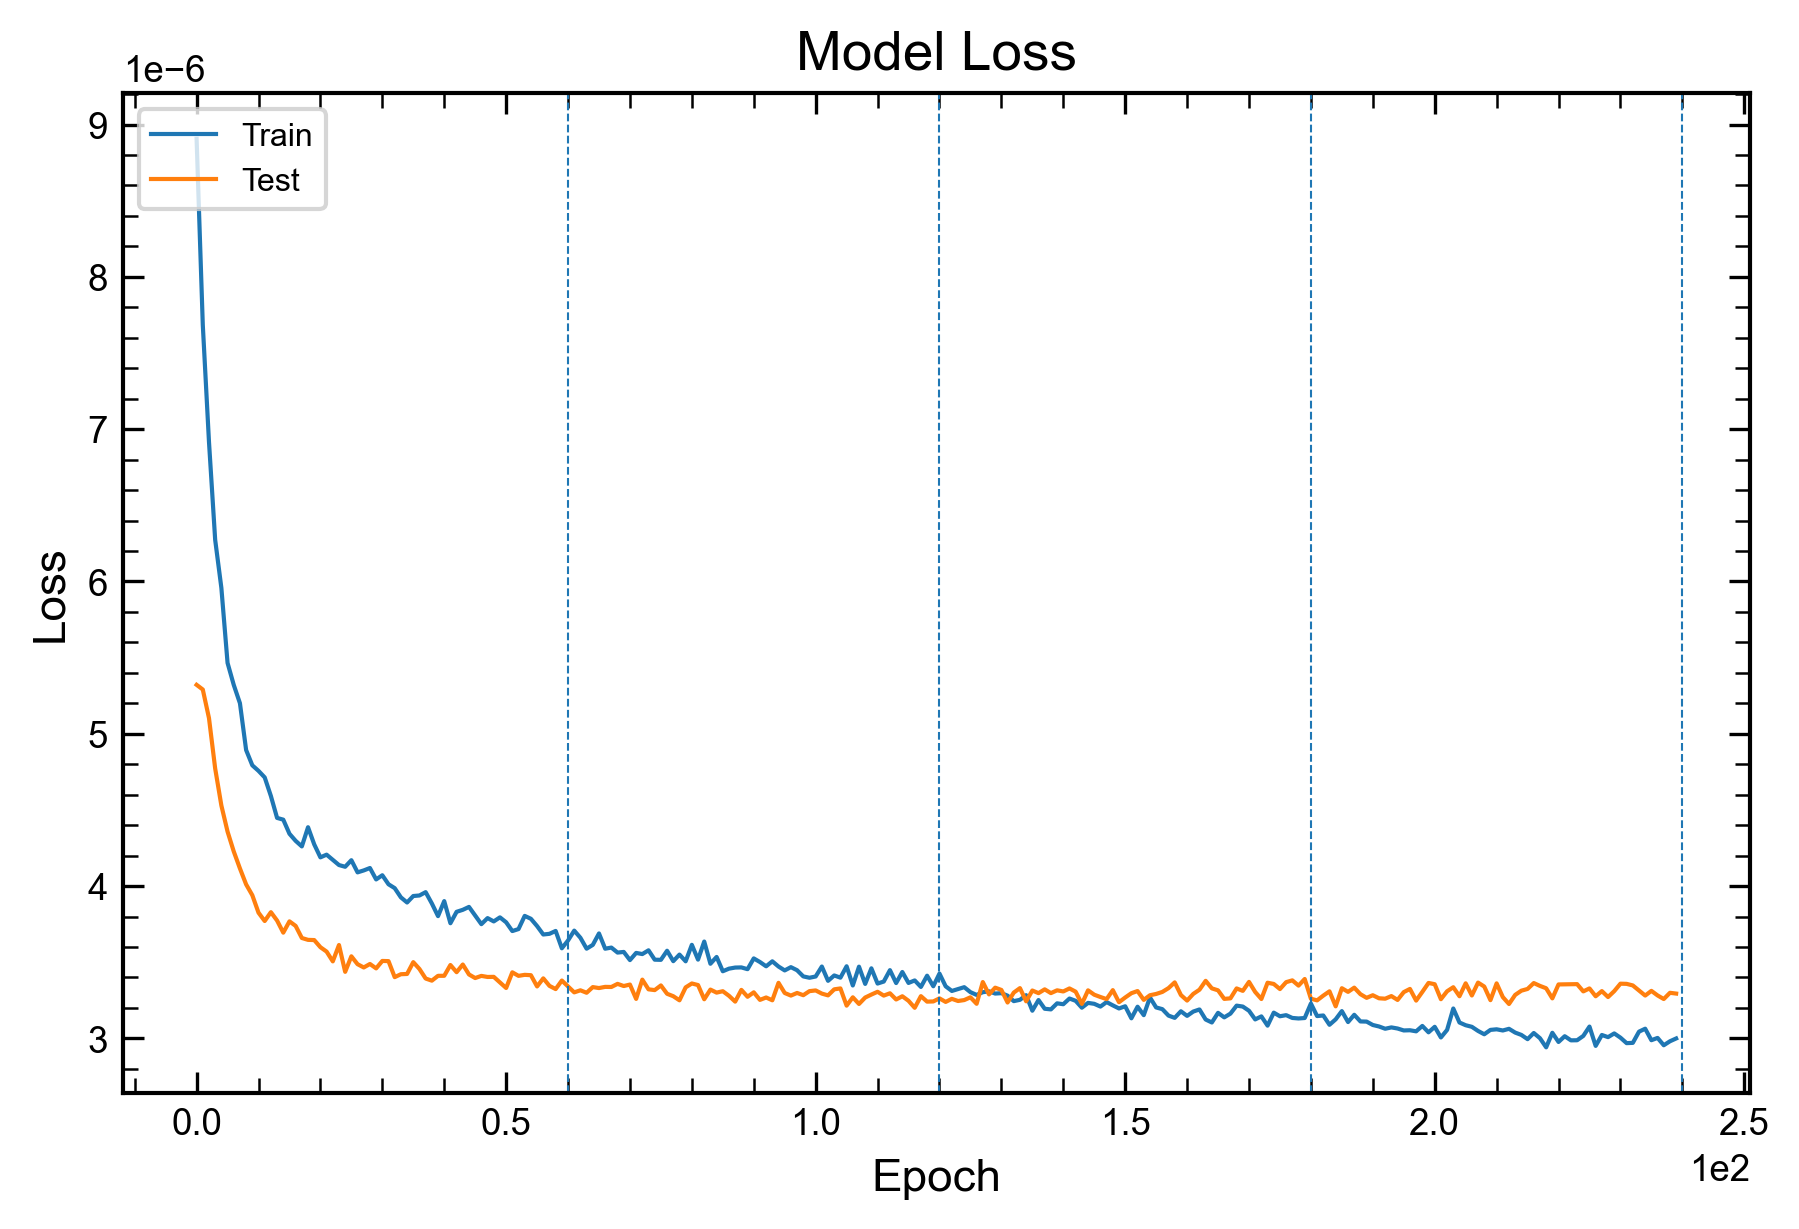
\includegraphics[width=0.8\textwidth]{loss_binary}
\begin{itemize}
  \item Should decrease
  \item Should not diverge
\end{itemize}
\end{frame}

\begin{frame}{The response}
  \centering 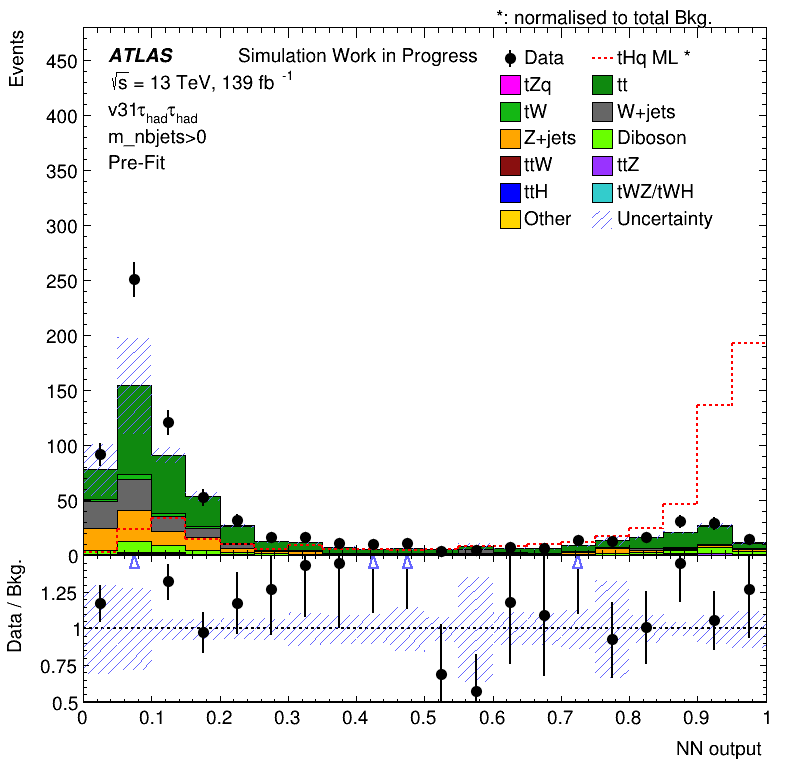
\includegraphics[width=0.6\textwidth]{response_binary}
  \begin{itemize}
    \item Seeing a separation is good
    \item Signal should be right
  \end{itemize}
\end{frame}

\section{\tZq difficulties}
\begin{frame}
    \begin{center}
        \Huge \tZq \\ Weakness in a binary separation
    \end{center}
\end{frame}

\begin{frame}{Response}
    \centering 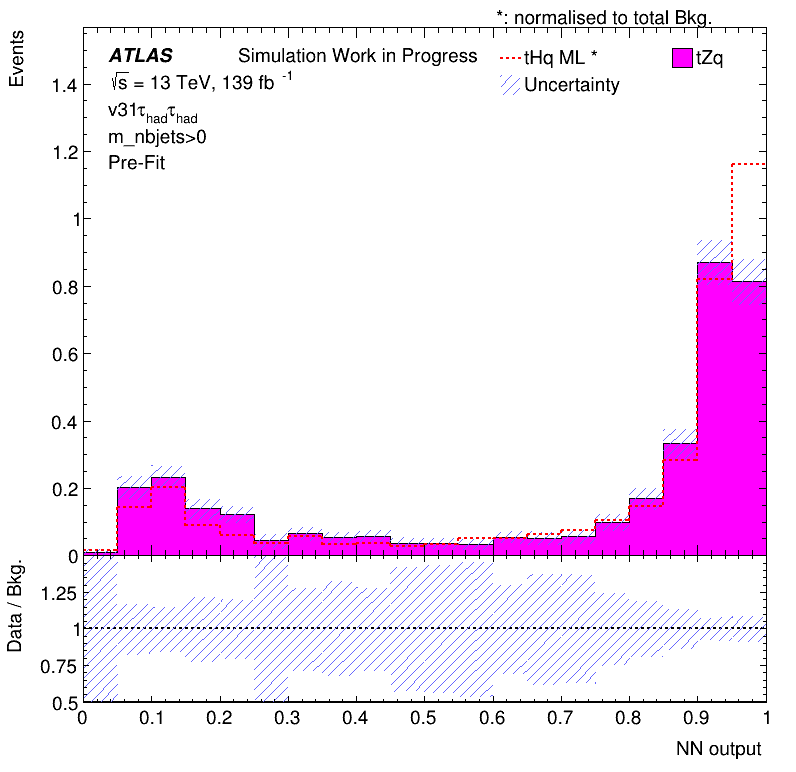
\includegraphics[width=0.81\textwidth]{tZq_problem}
\end{frame}
\section{Categorical}
\begin{frame}
    \begin{center}
        \Huge Categorical Neural Networks
    \end{center}
\end{frame}

\begin{frame}{The idea of categorical neural networks}
    \begin{itemize}
        \item \Large Difficult backgrounds $\rightarrow$ additional targets
    \end{itemize}
\end{frame}

\begin{frame}{Target handling}
    \begin{itemize}
        \item Using One-Hot-Encoding
        \vspace{0.23cm}
        \item Vector instead of target
        \vspace{0.23cm}
        \item Target values get translated to vector component
    \end{itemize}
    \vspace{0.23cm}
    \begin{equation*}
    \tHq = \begin{bmatrix}
           0 \\
           0 \\
           1
         \end{bmatrix}
    \tZq = \begin{bmatrix}
           1 \\
           0 \\
           0
         \end{bmatrix}
    Background = \begin{bmatrix}
           0 \\
           1 \\
           0
         \end{bmatrix}
    \end{equation*}
\end{frame}

\begin{frame}{Binary final node - Sigmoid}
    \begin{columns}
        \begin{column}{0.65\textwidth}
            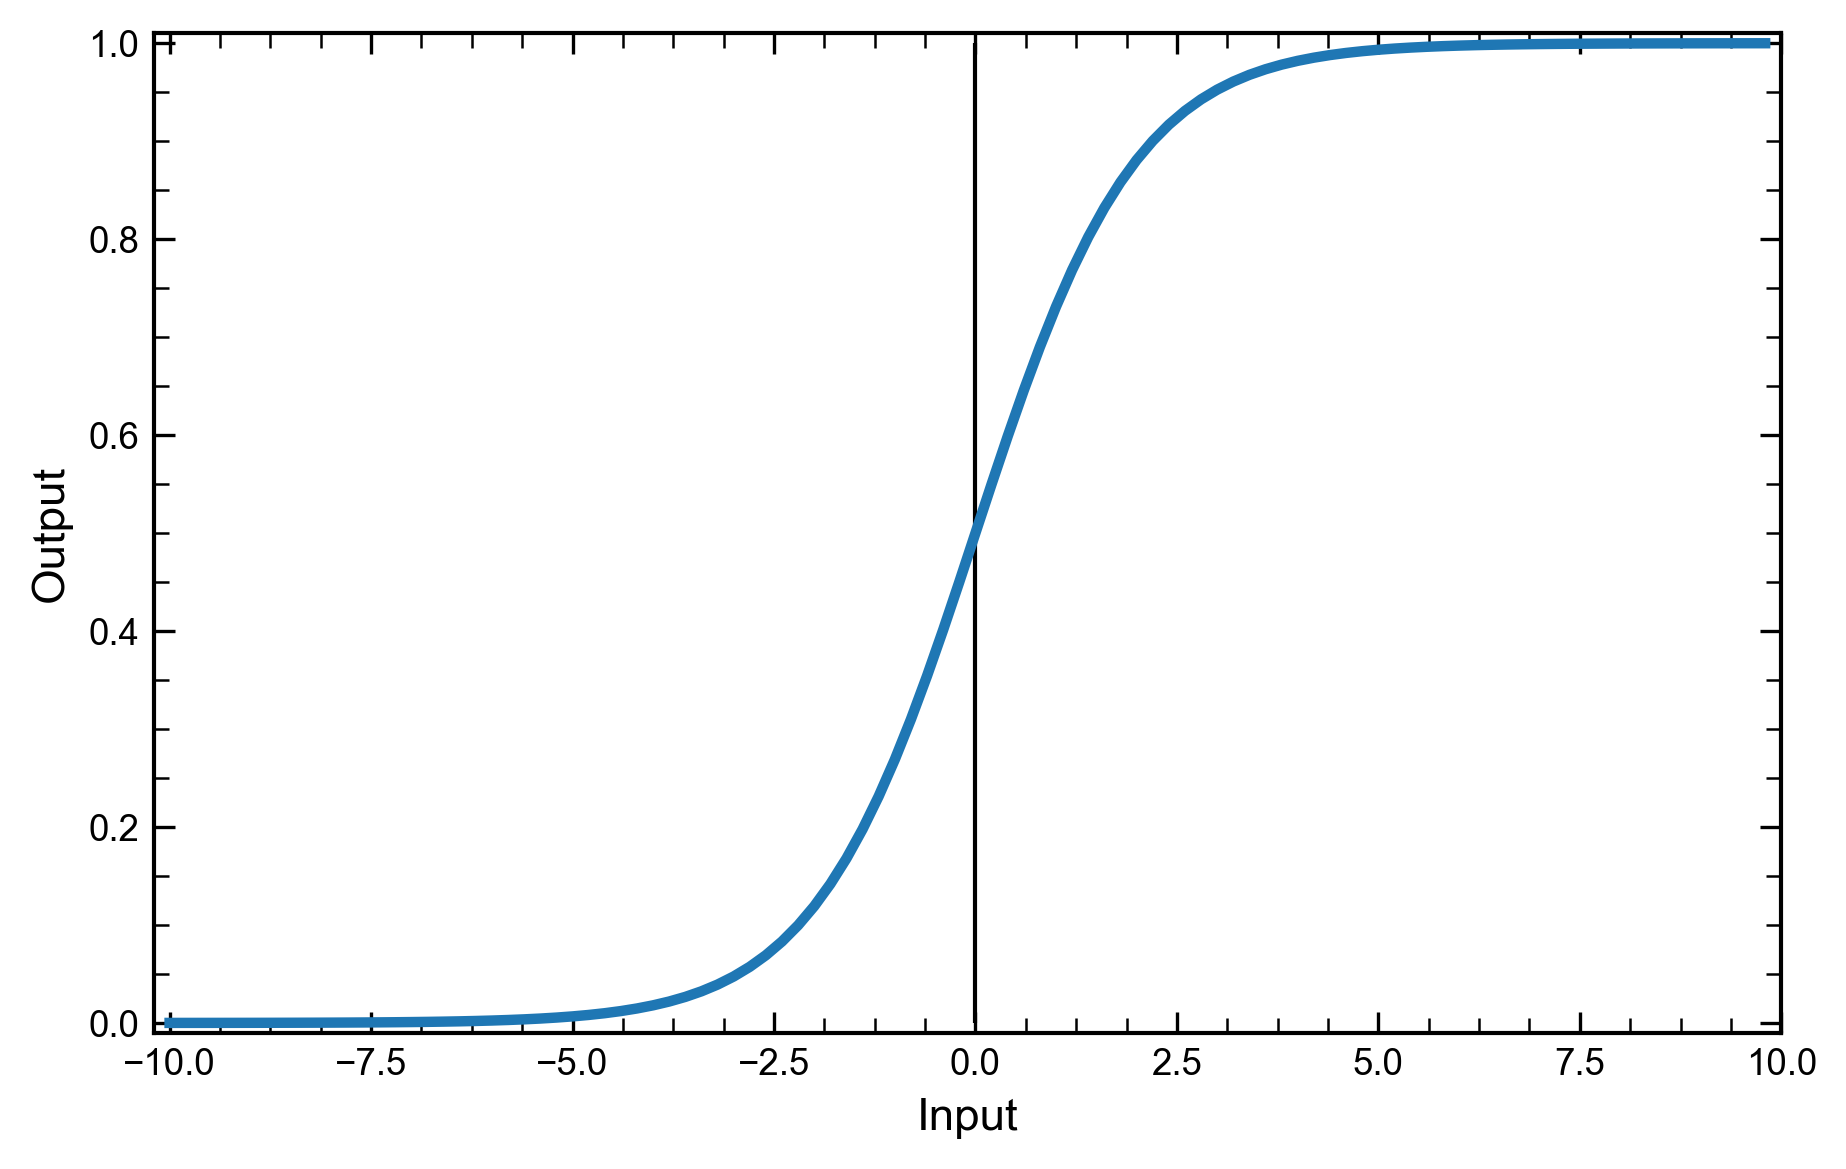
\includegraphics[width=\textwidth]{sigmoid}
        \end{column}
        \begin{column}{0.5\textwidth}
            \begin{itemize}
                \item Bounded, differentiable
                \item Allows for backpropagation
                \item Assigning a single output value $\in (0,1)$
            \end{itemize}
            \begingroup
            \large
            \begin{equation*}
                \frac{1}{1+e^{-s_i}}
            \end{equation*}
            \endgroup
        \end{column}
    \end{columns}
    \begin{itemize}
        \color{red}
        \item Expects only one input value
    \end{itemize}
\end{frame}

\begin{frame}{Categorical final node - Softmax}
    \begin{columns}
        \begin{column}{0.5\textwidth}
            \begingroup
            \huge
            \begin{equation*}
                f(s)=\frac{e^{s_i}}{\sum_j^c e^{s_j}}
            \end{equation*}
            \endgroup
        \end{column}
        \begin{column}{0.5\textwidth}
            \begin{itemize}
                \item Takes an input vector equal to the number of targets
                \vspace{0.1cm}
                \item Sum of vector components is 1
                \vspace{0.1cm}
                \item normalises output to a probability distribution
            \end{itemize}
        \end{column}
    \end{columns}
\end{frame}

\begin{frame}{Loss function - Crossentropy}
    \begin{columns}
        \begin{column}{0.5\textwidth}
            \begin{block}{Binary Crossentropy}
                \begin{equation*}
                    Loss = - \sum_{i=1} y_i \log \hat{y}_i =
                \end{equation*}
                \begin{equation*}
                    -y_1 \log \hat{y_1} - (1-y_1) \log (1-\hat{y}_1)
                \end{equation*}
                \begin{itemize}
                    \item Measures model quality for two classes
                \end{itemize}
            \end{block}
        \end{column}
        \begin{column}{0.5\textwidth}
            \begin{block}{Categorical Crossentropy}
                \begin{equation*}
                    Loss = - \sum_{i=1} y_i \log \hat{y_i}
                \end{equation*}
                \begin{itemize}
                    \item Measures model quality for multiple classes
                \end{itemize}
            \end{block}
        \end{column}
    \end{columns}
\end{frame}

\begin{frame}{Hyperparameters}
    \begin{table}[]
    \begin{tabular}{|l|l|}
    \hline
    Hyperparameter          &     Setting              \\ \hline
    Model                   &     Categorical          \\ \hline
    Nodes                   &     120                  \\ \hline
    Layers                  &     6                    \\ \hline
    Dropout                 &     0.65                 \\ \hline
    Batchnormalisation      &     On                   \\ \hline
    Activation              &     elu                  \\ \hline
    Output activation       &     Softmax              \\ \hline
    Batch size              &     1000                 \\ \hline
    Optimisation            &     Adam                 \\ \hline
    Weight Initialisation   &     Lecun Normalisation  \\ \hline
    K-folds                 &     4                    \\ \hline
    \end{tabular}
    \end{table}
\end{frame}

\begin{frame}{Results}
    \begin{columns}
        \begin{column}{0.5\textwidth}
          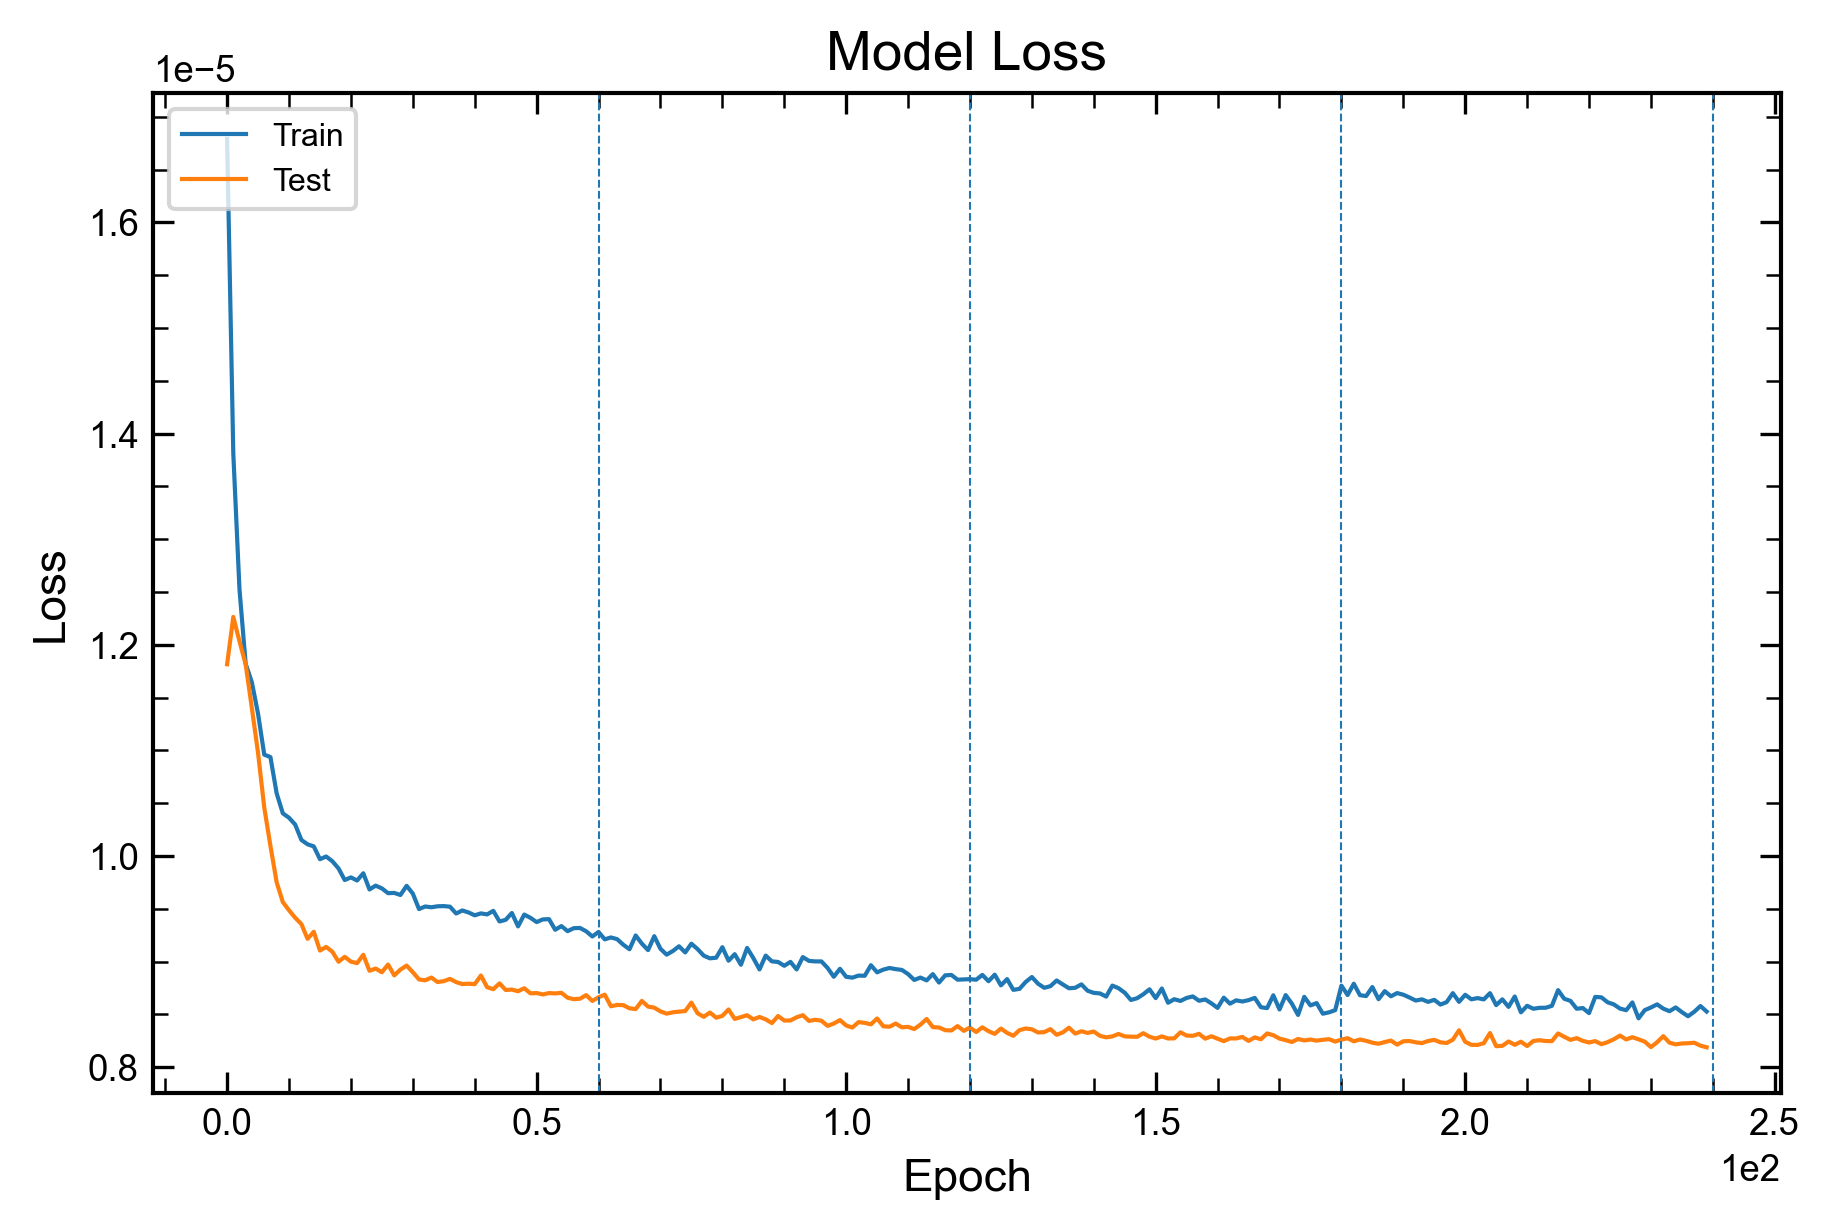
\includegraphics[width=0.8\textwidth]{losses_cat}
          \begin{itemize}
            \item Stable training
            \item Good AUC
          \end{itemize}
        \end{column}
        \begin{column}{0.5\textwidth}
          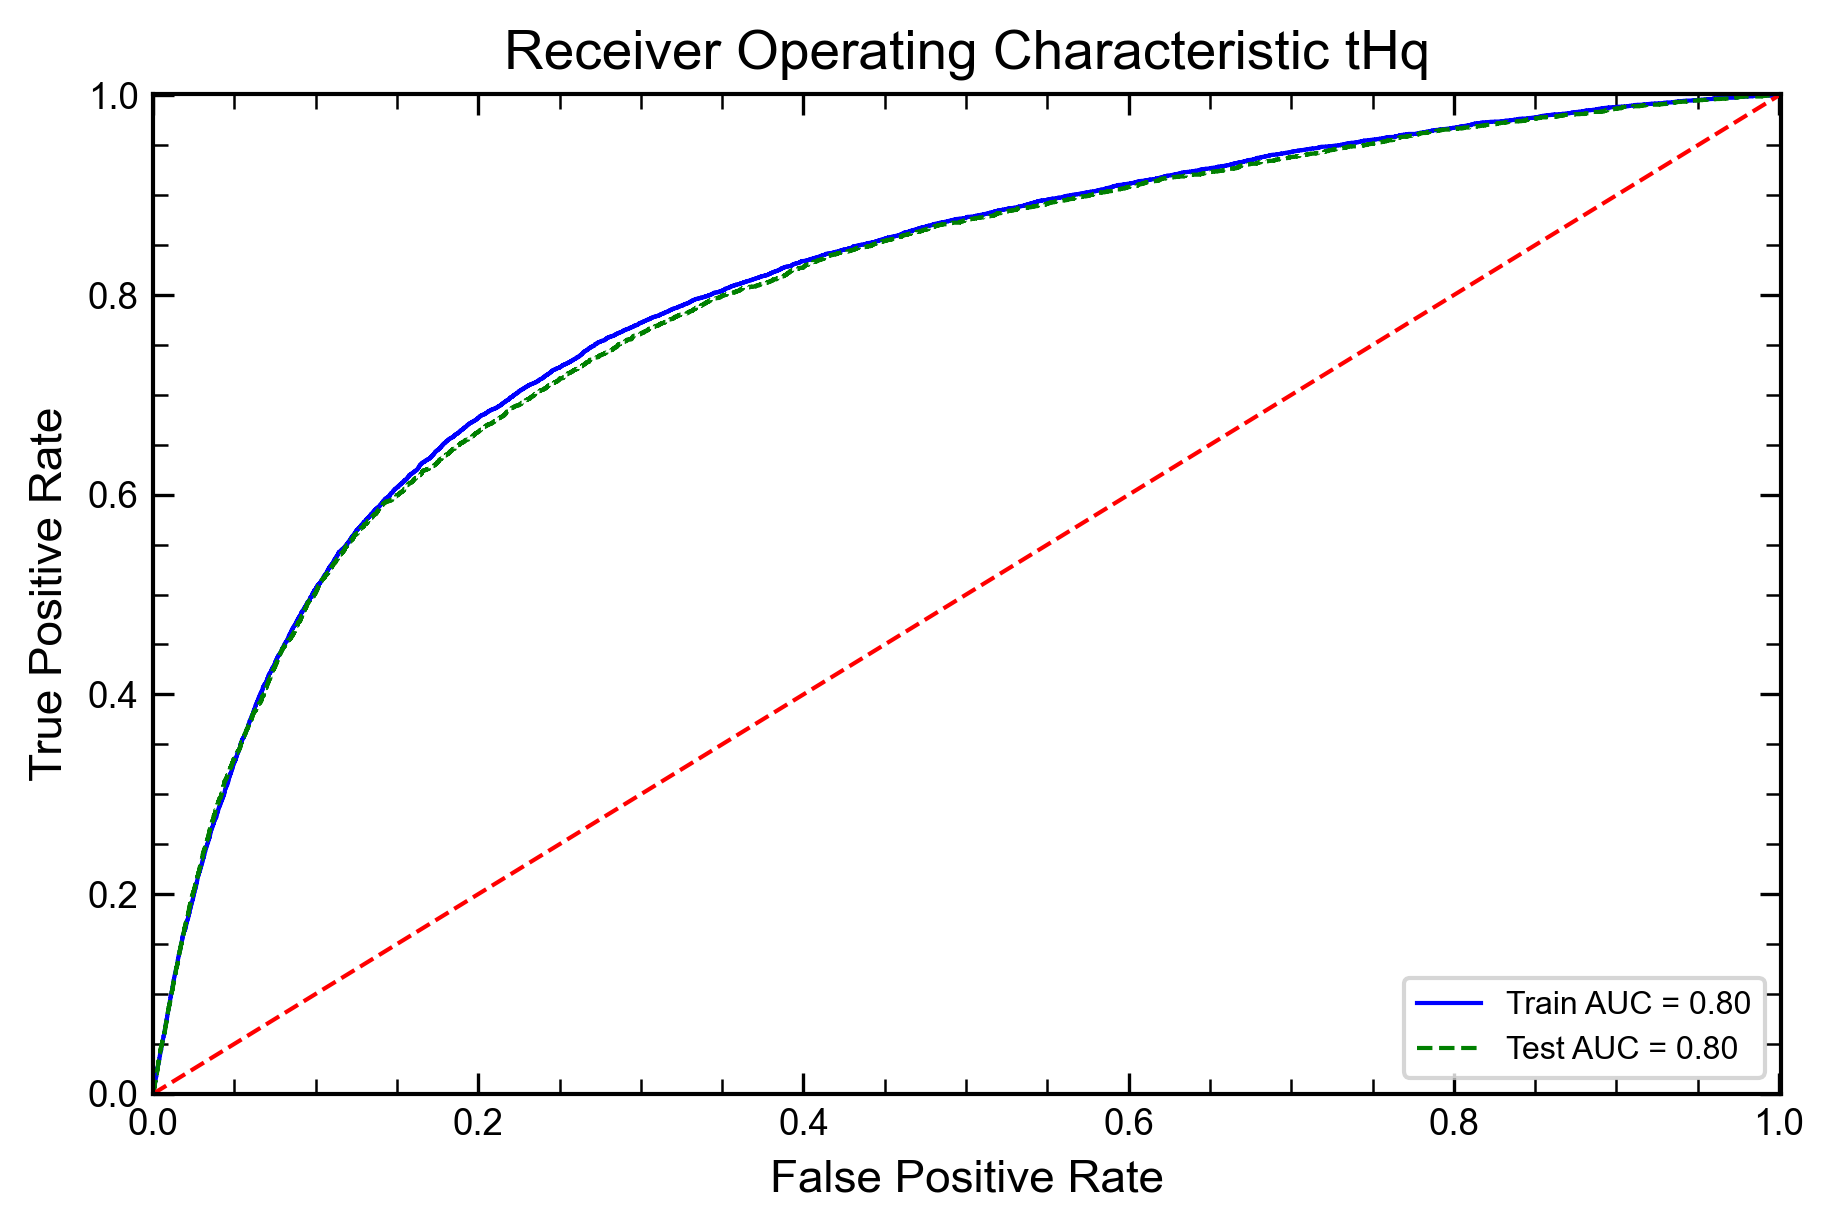
\includegraphics[width=0.8\textwidth]{ROC_cat}
          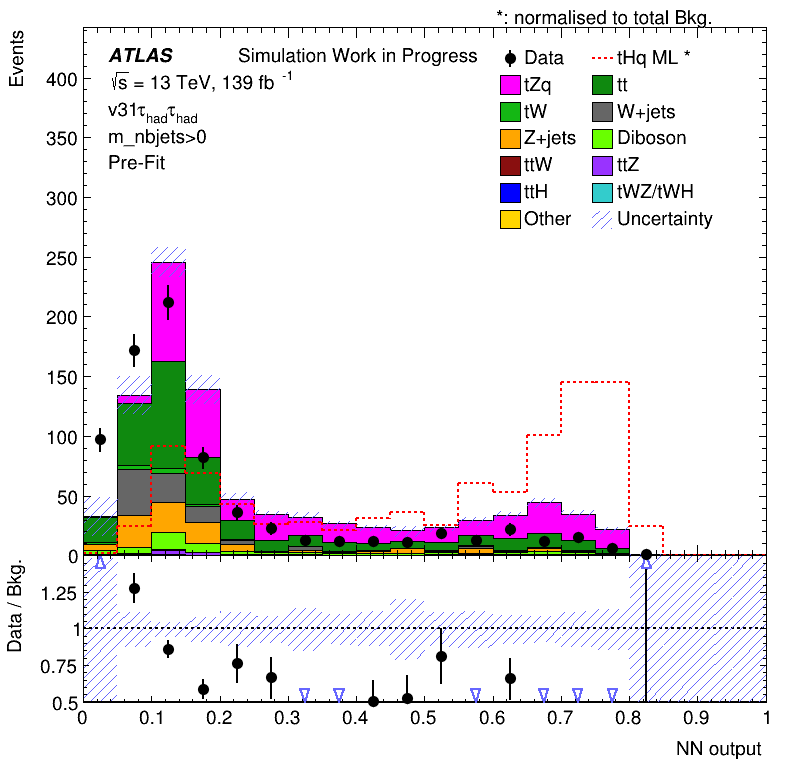
\includegraphics[width=0.8\textwidth]{response_cat}
        \end{column}
    \end{columns}    
\end{frame}

\begin{frame}{Response}
      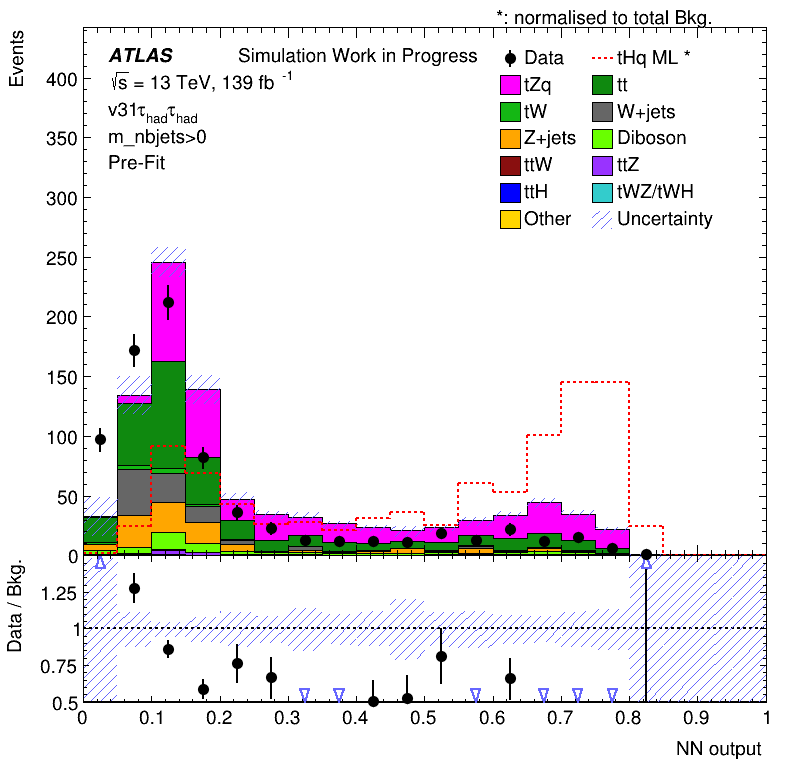
\includegraphics[width=0.75\textwidth]{response_cat}
\end{frame}

\begin{frame}{Additional responses}
  \begin{columns}
    \begin{column}{0.5\textwidth}
      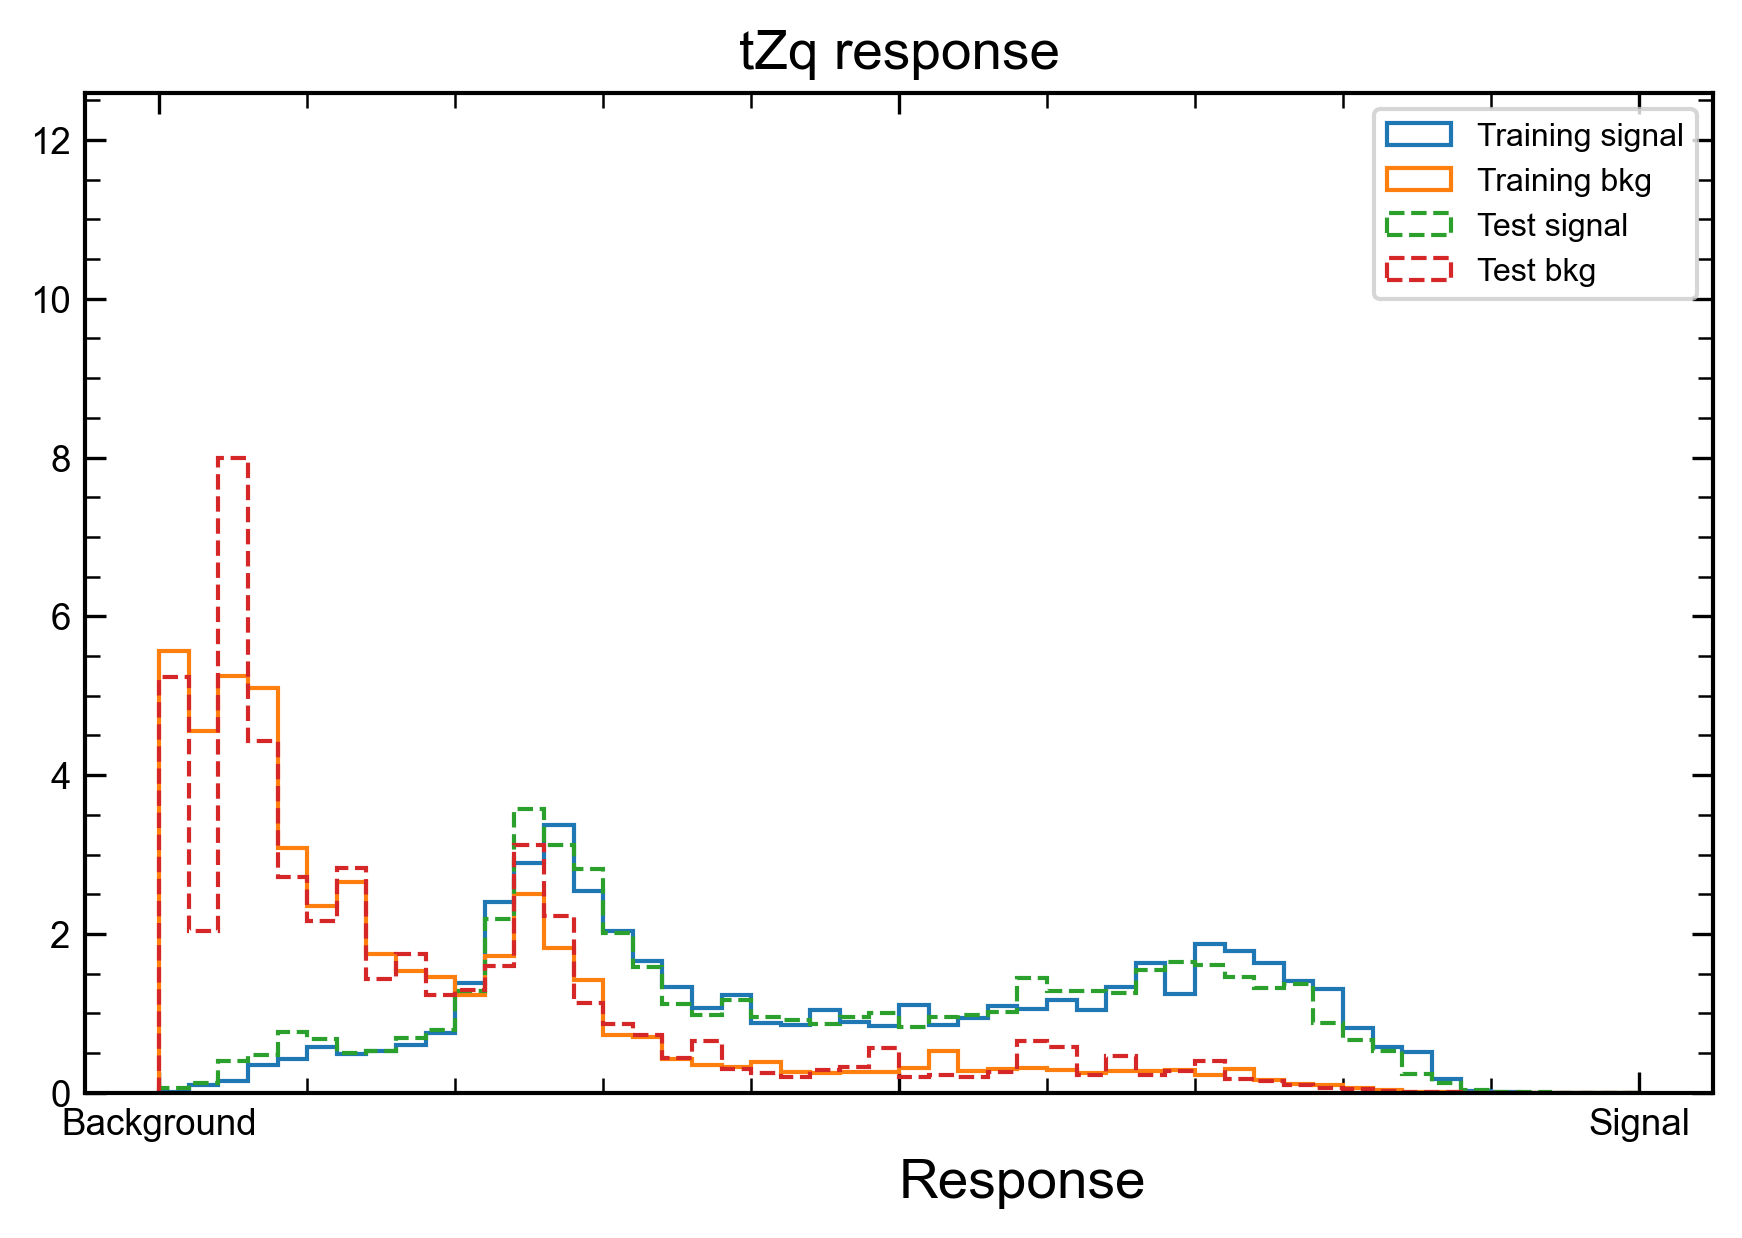
\includegraphics[width=0.8\textwidth]{resp1}
      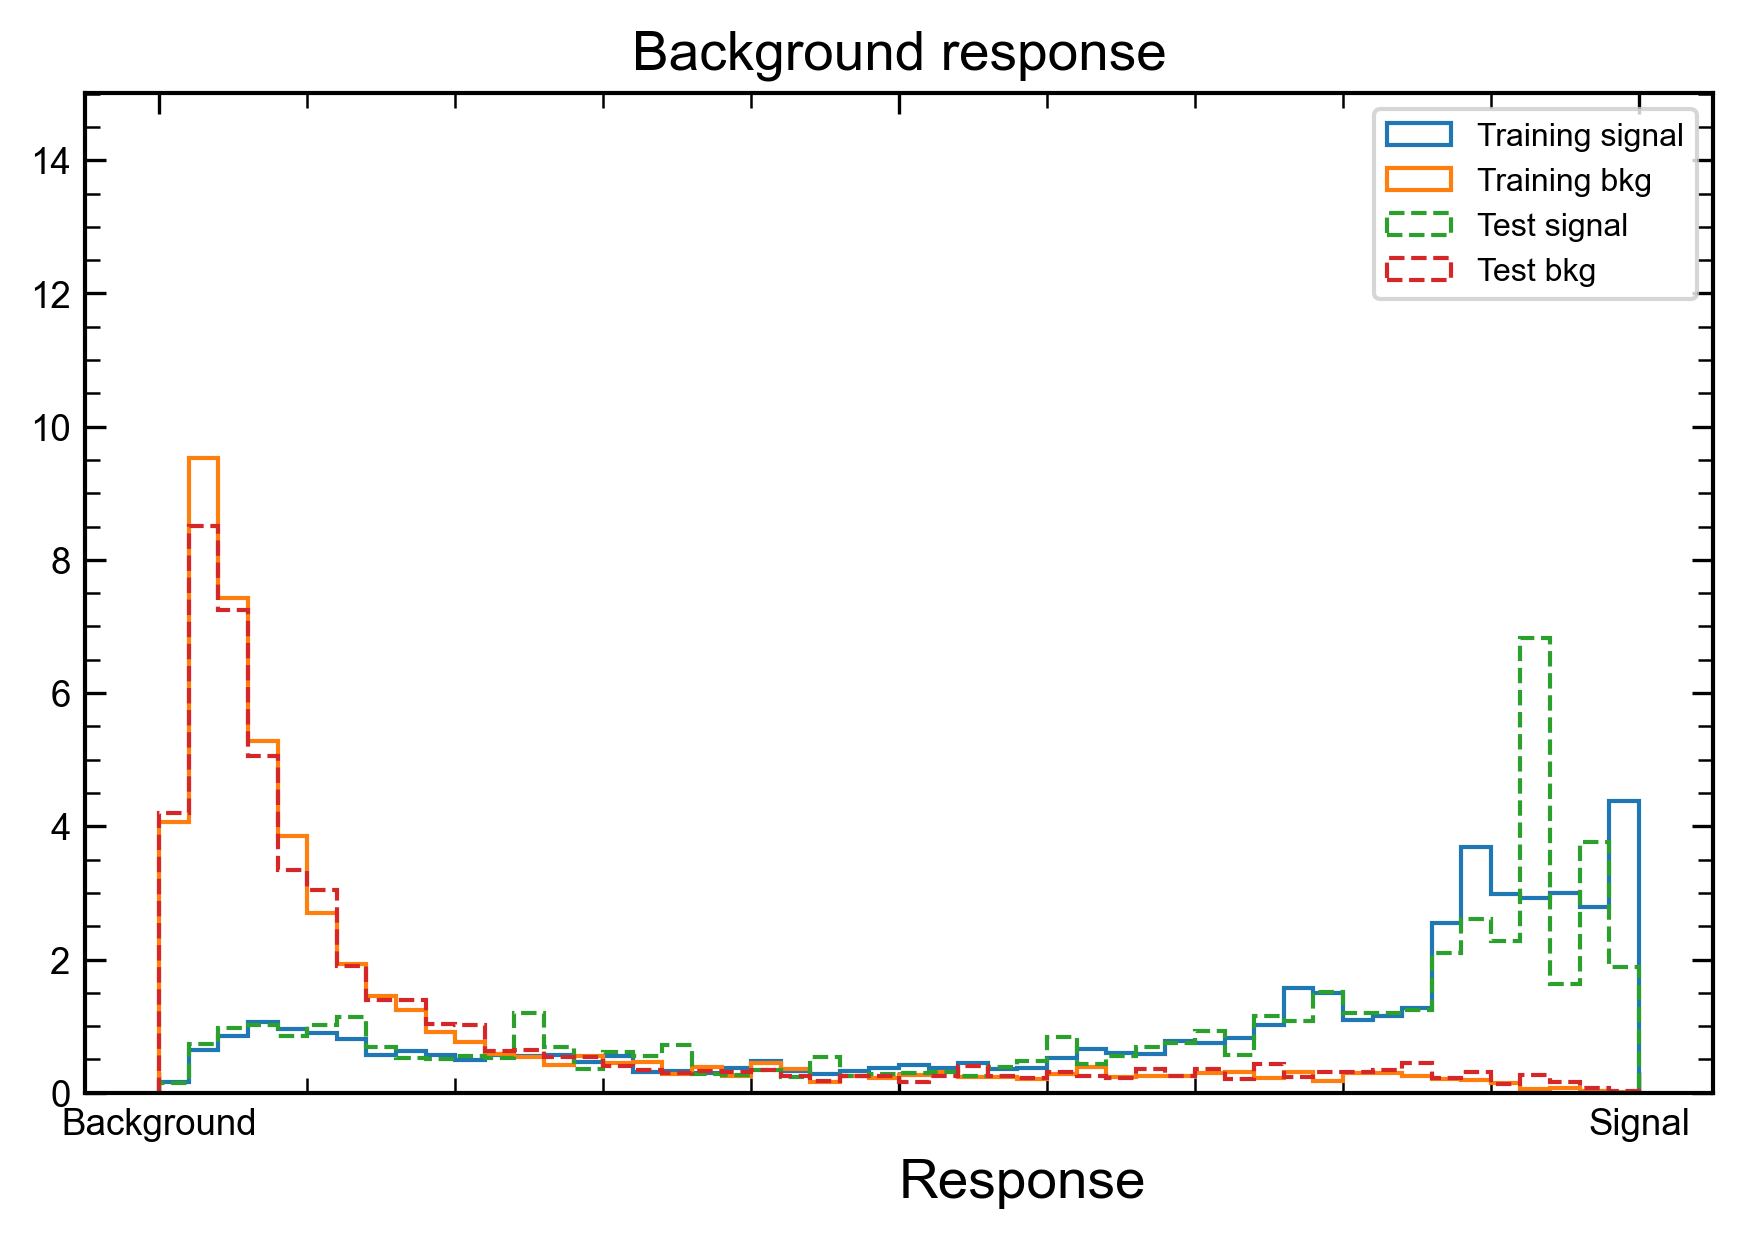
\includegraphics[width=0.8\textwidth]{resp2}
    \end{column}
    \begin{column}{0.5\textwidth}
      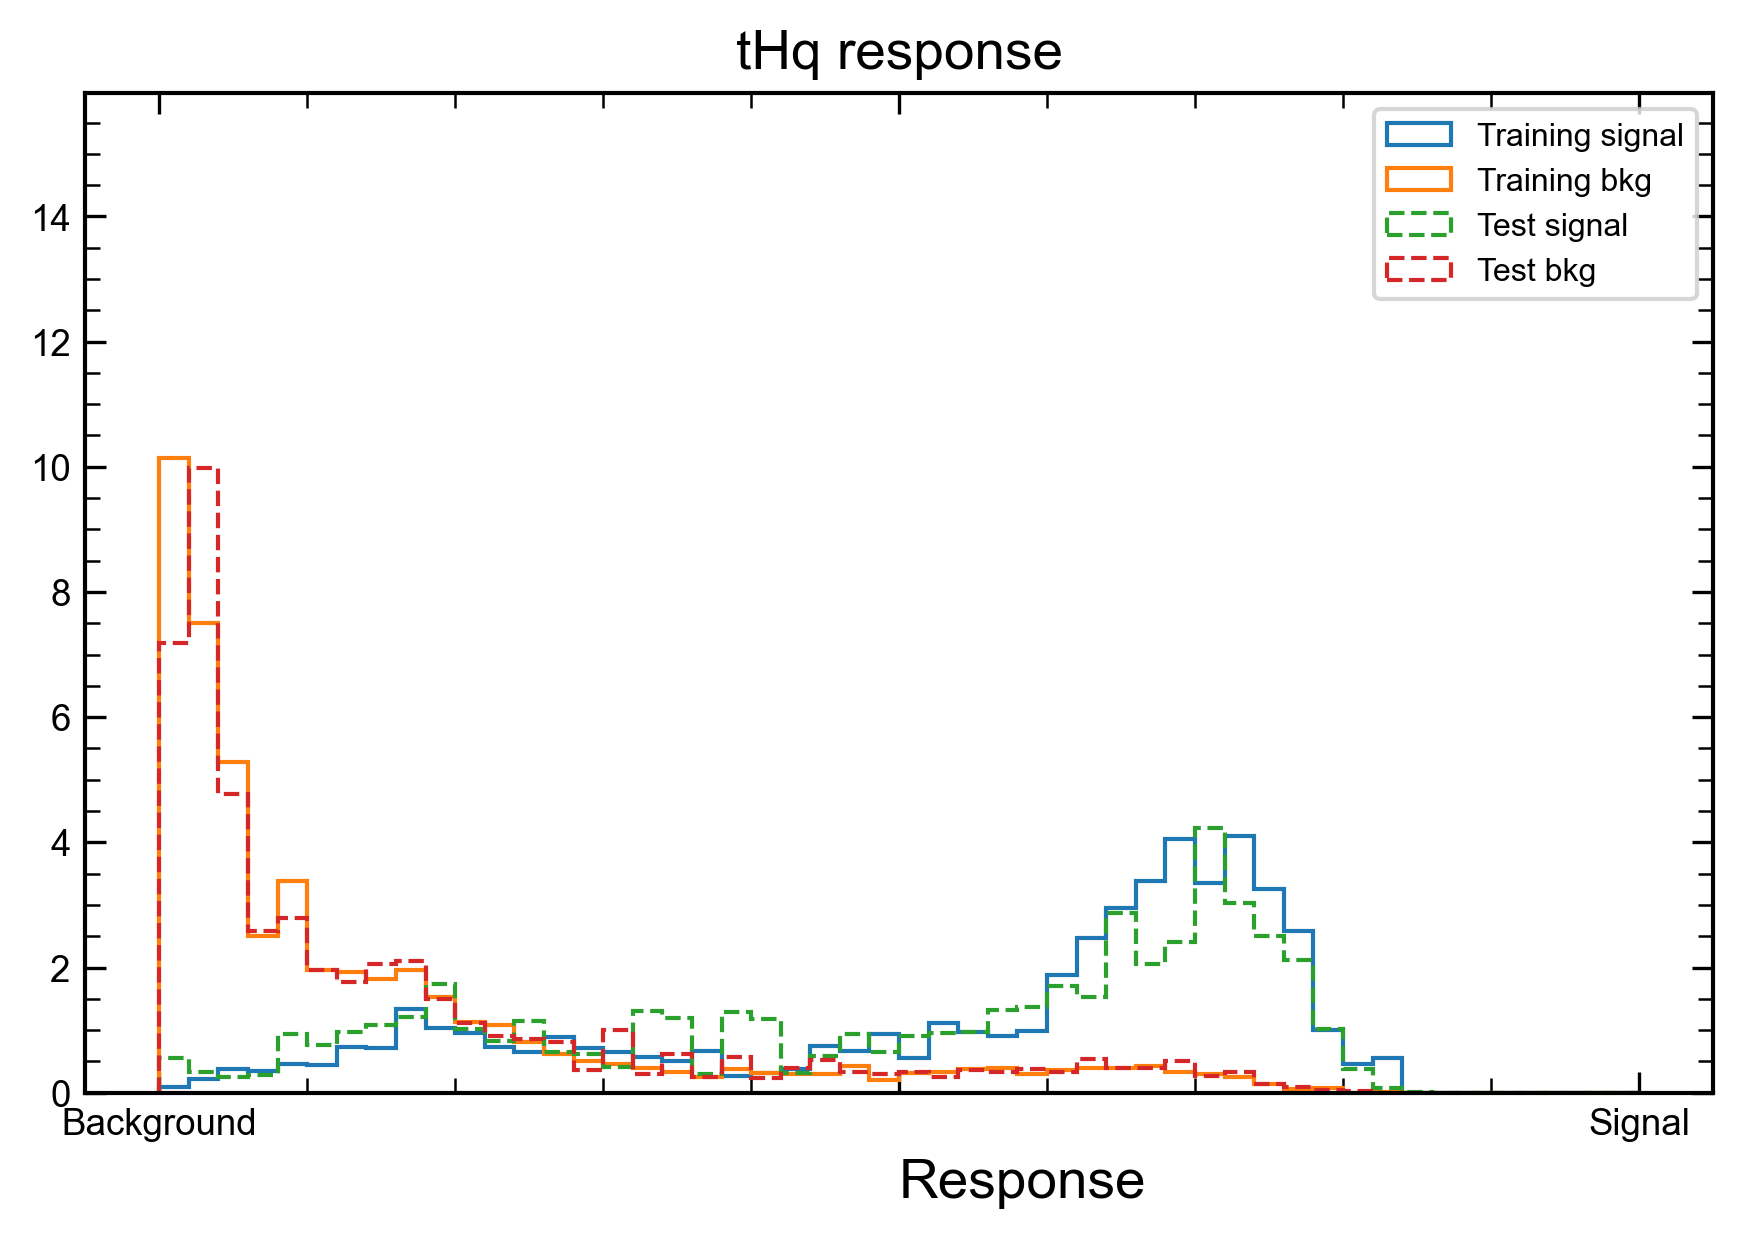
\includegraphics[width=0.8\textwidth]{resp3}
      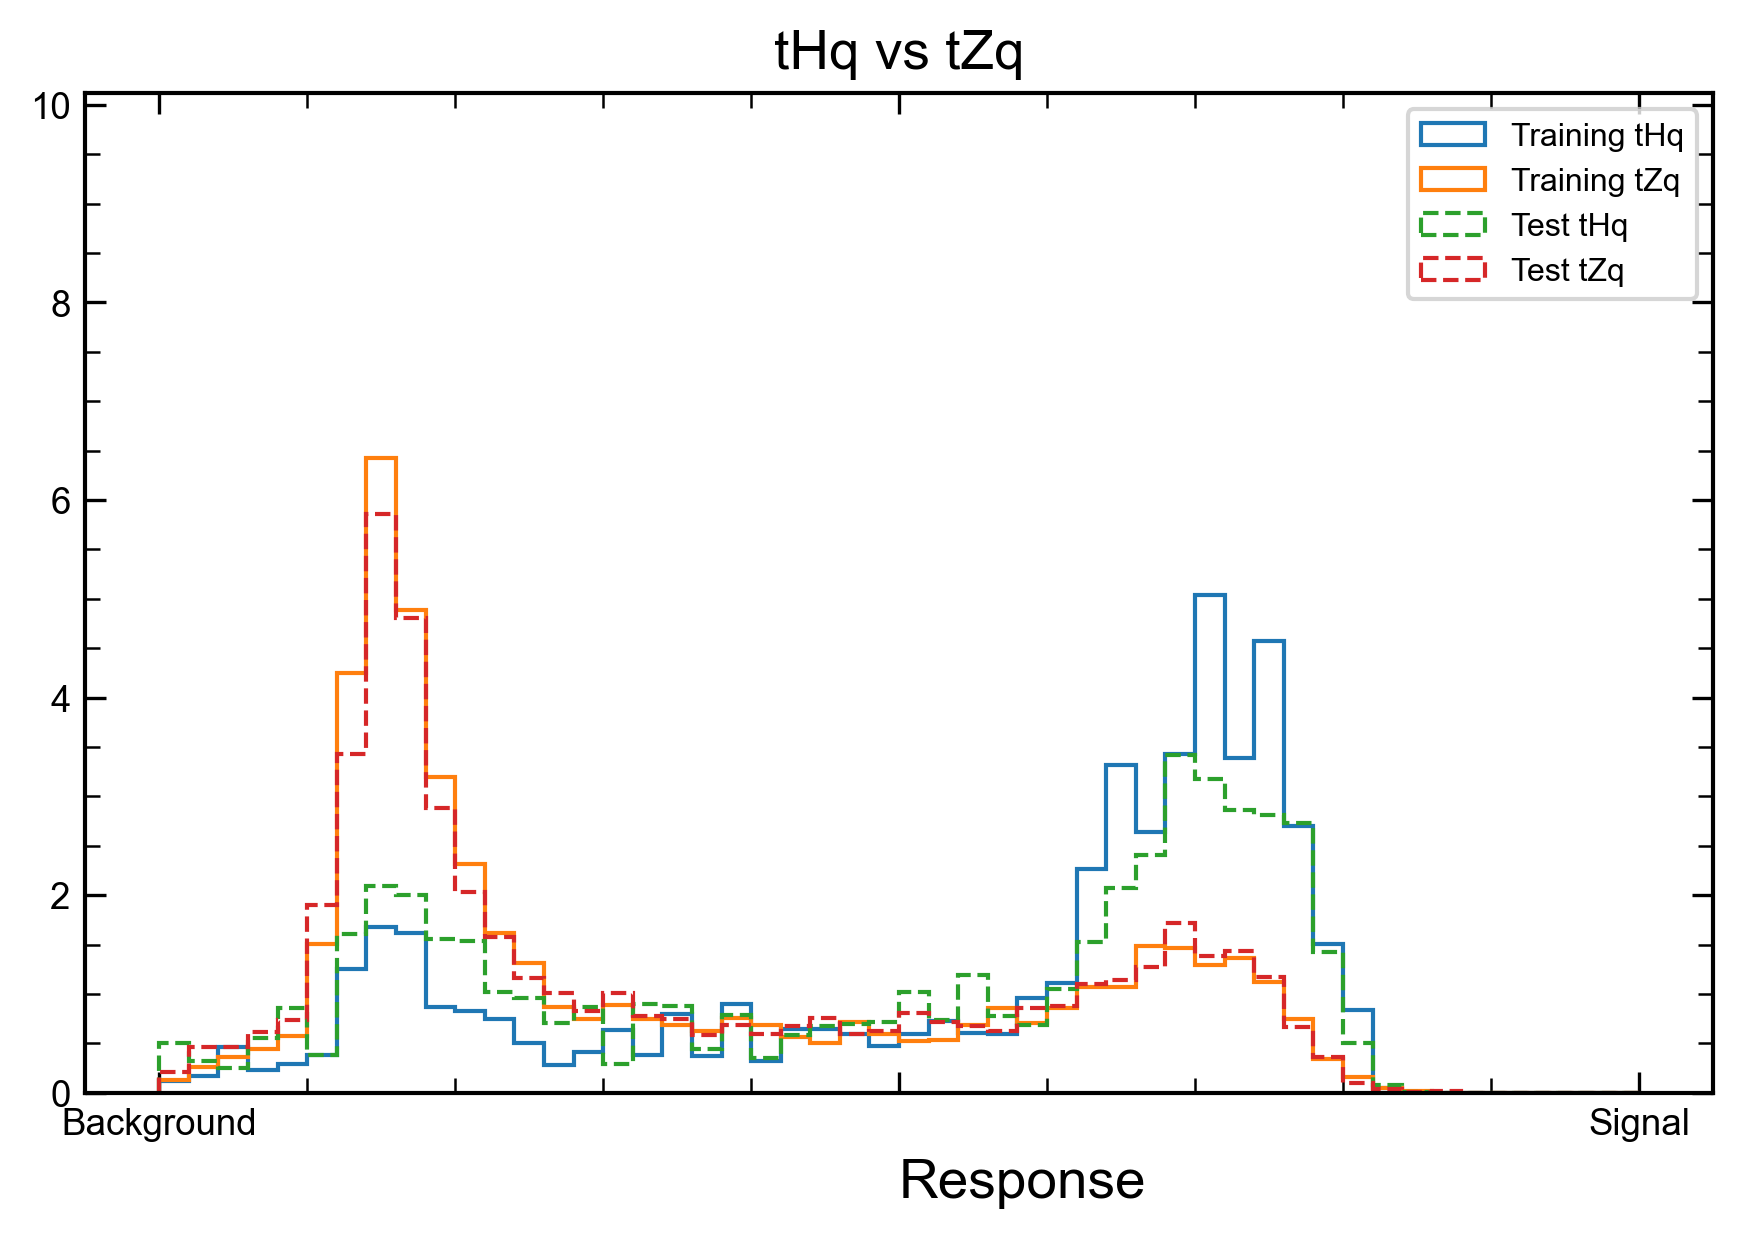
\includegraphics[width=0.8\textwidth]{resp4}
    \end{column}
  \end{columns}    
\end{frame}



\section{Conclusion}

\begin{frame}{Stacking two networks}
  \begin{columns}
    \begin{column}{0.65\textwidth}
      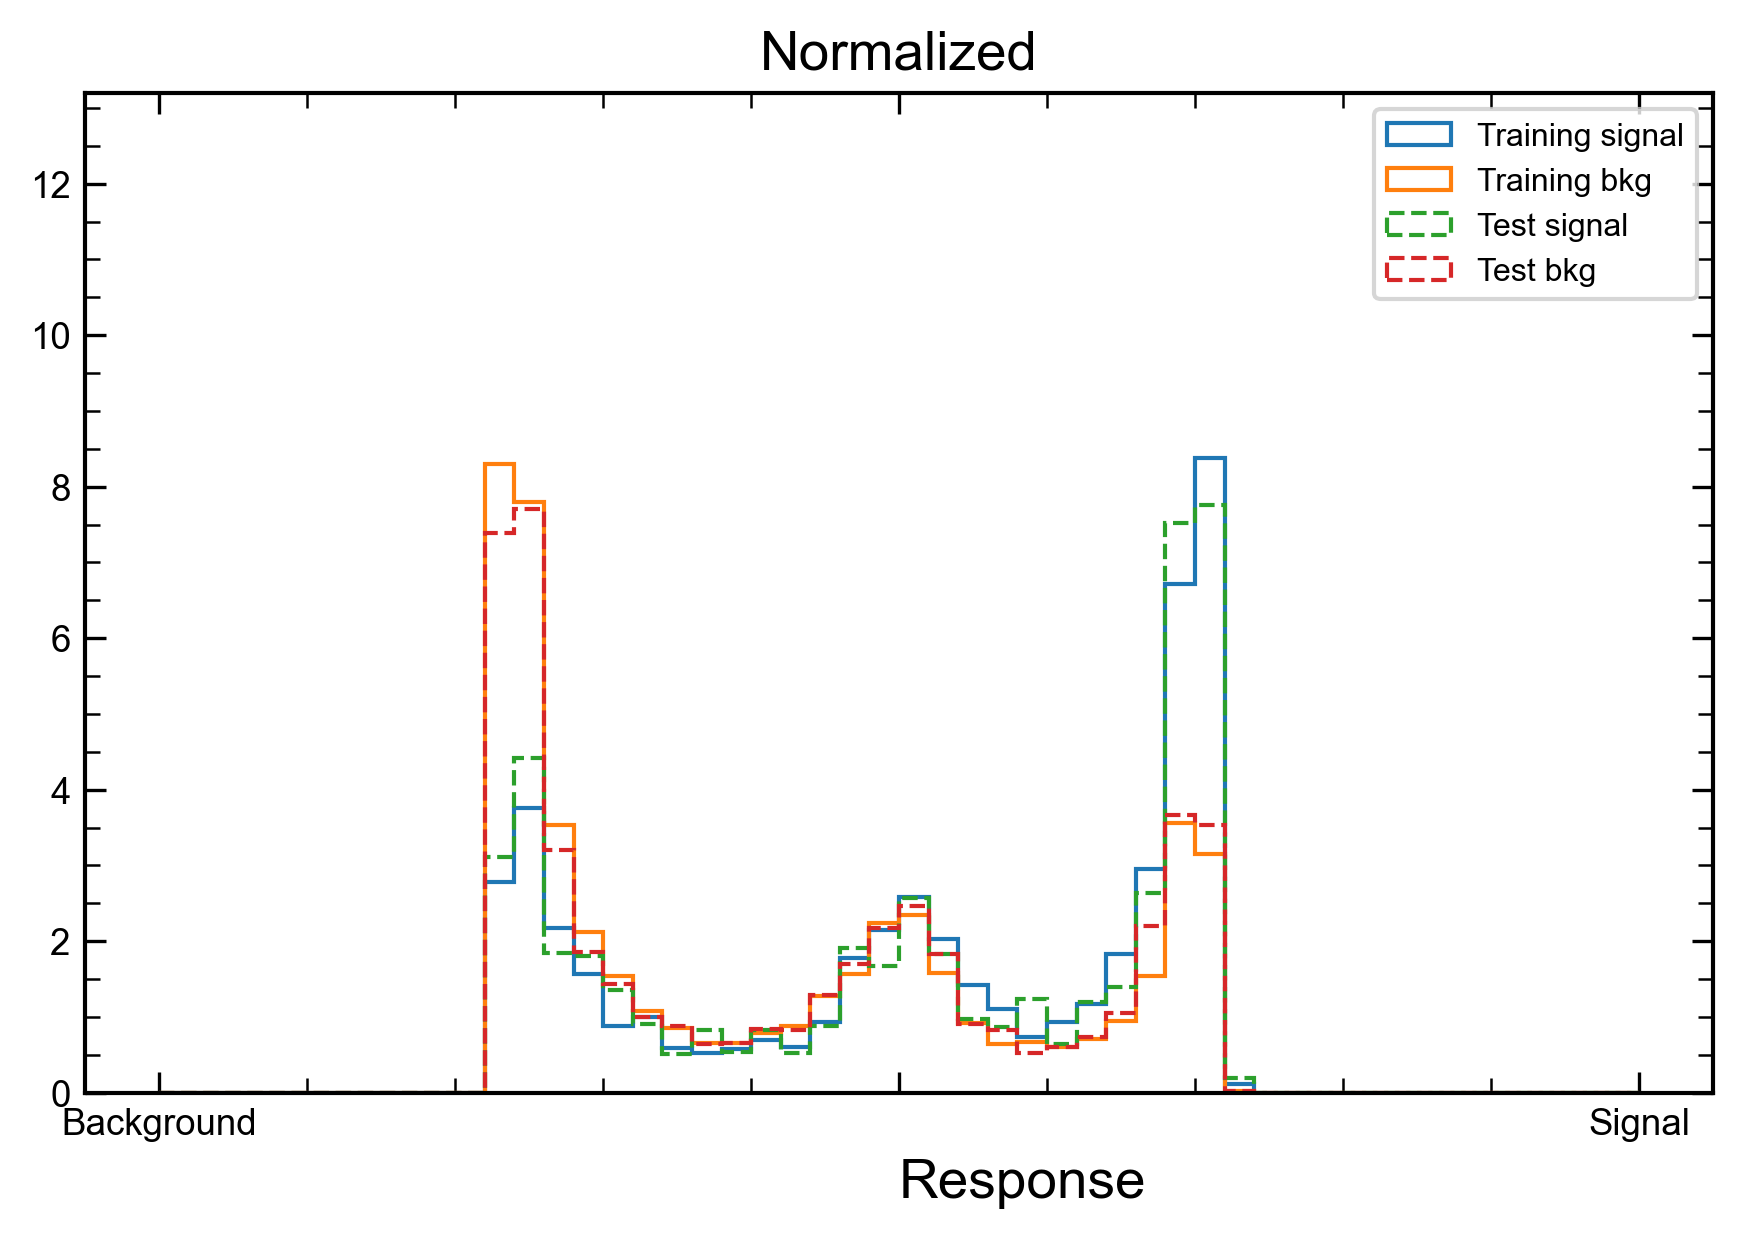
\includegraphics[width=\textwidth]{stacked}
    \end{column}
    \begin{column}{0.35\textwidth}
      \begin{itemize}
        \item Stacking two networks for additional \tZq separation
        \item Recently tested
        \item Not obviously worth the effort
      \end{itemize}
    \end{column}
  \end{columns}
\end{frame}

\begin{frame}{Conclusion}
\begin{itemize}
  \item Signal-like backgrounds are a weakness of binary classifiers
  \vspace{0.25cm}
  \item Categorical neural networks are a promising approach and easy to implement 
  \vspace{0.25cm}
  \item The pollution of the signal by similar backgrounds is visibly decreased
  \vspace{0.25cm}
  \item Combining the likelihoods could produce a more potent classifier
  \vspace{0.25cm}
  \item Better Higgs mass reconstruction promises even more improvement
\end{itemize}
\end{frame}



%
%

  

\end{document}